\chapter{New Revolutions in Particle Physics: Basic Concepts}

These notes follow Lecture 1 of Leonard Susskind's \emph{Particle Physics 1: Basic Concepts}. They are written as a logical history rather than a strict chronology, in the same spirit as the lecture itself, and the curation of the lecture materials is due to LazyingArt LLC. The organizing question is very old and very hard to get away from: is nature built from discrete things, or is it continuous? From that question we are led, in order, to chemistry, radioactivity, light as a classical wave, light as a quantum of energy, relativity, natural units, and finally to the practical logic of particle physics: shorter wavelength means larger momentum and energy, and therefore larger machines.

\section{Discreteness, Continuity, and the First Chemical Evidence}

Particle physics begins here not with a list of particles but with a contrast of pictures. One picture says that matter comes in indivisible units. The ancient name for such a unit was the atom; in the broad spirit of the lecture we may simply call such units particles. The opposite picture says that matter is not built from localized lumps at all, but is continuously distributed. In that language one speaks of fields: functions on space, such as a density field, or the electric and magnetic fields.

Already at the start one should be careful. The lecture does not treat this as a contest in which one side simply wins. Quantum mechanics will eventually force us to say that the particle picture and the field picture are both indispensable, and neither is fully adequate on its own. But before we get there, we want evidence.

The first serious evidence for discreteness is presented through chemistry. Dalton noticed that the mass of a fixed number of molecules of a substance is, to a good approximation, an integer multiple of the mass of the same number of hydrogen molecules. The striking point is not exact arithmetic perfection; it is the near-integral pattern. Not three halves, not \(\pi\), but integers. This is the kind of regularity that suggests building blocks.

From the modern point of view we can see why this pattern was such a strong clue. Ordinary matter is made of atoms, and the mass of an atom is overwhelmingly concentrated in protons and neutrons, with the electrons contributing only a very small correction. Protons and neutrons have nearly the same mass, while the nucleus of hydrogen contains just one proton. So, to a first approximation, the mass of ordinary matter is counted in units of proton-or-neutron mass, and Dalton's integer pattern becomes intelligible. The lecture is careful here: the pattern is approximate, not exact, but the approximation is good enough to reveal discreteness.

By the end of nineteenth-century chemistry, the elements themselves were treated as the elementary building blocks. That picture was about to break.

\section{Radioactivity and the First Particle Beam}

Radioactivity appears in the lecture as the first genuinely particle-physics-style experiment. Becquerel notices first that radioactive material affects a photographic plate as if some radiation were present. He then buries the source inside a block of lead, drills a narrow hole, and lets whatever emerges travel toward a photographic plate. The hole collimates the emission, so what had been a diffuse effect becomes a beam.

\begin{figure}[h]
\centering
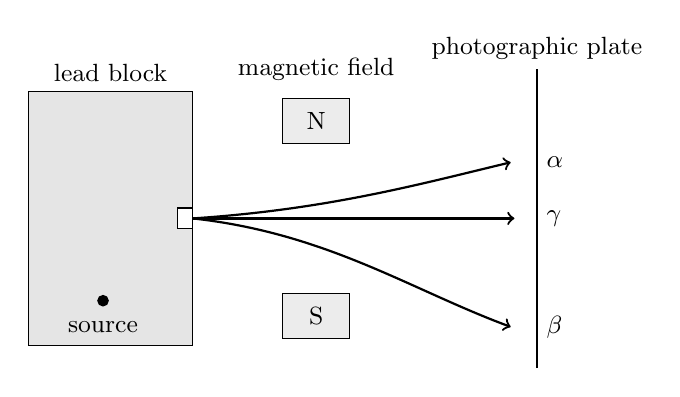
\begin{tikzpicture}[scale=0.95]
\draw[fill=gray!20] (0,-1.7) rectangle (2.2,1.7);
\draw[fill=white] (2.0,-0.14) rectangle (2.2,0.14);
\draw[fill=black] (1.0,-1.1) circle (0.07);
\node at (1.0,-1.45) {\small source};

\draw[thick] (6.8,-2.0) -- (6.8,2.0);
\node[above] at (6.8,2.0) {\small photographic plate};

\draw[fill=gray!15] (3.4,1.0) rectangle (4.3,1.6);
\draw[fill=gray!15] (3.4,-1.6) rectangle (4.3,-1.0);
\node at (3.85,1.3) {\small N};
\node at (3.85,-1.3) {\small S};

\draw[thick,->] (2.2,0.0) -- (6.5,0.0);
\draw[thick,->] (2.2,0.0) .. controls (4.0,0.12) and (5.2,0.45) .. (6.45,0.75);
\draw[thick,->] (2.2,0.0) .. controls (4.0,-0.2) and (5.1,-0.95) .. (6.45,-1.45);

\node[right] at (6.8,0.75) {\small \(\alpha\)};
\node[right] at (6.8,0.0) {\small \(\gamma\)};
\node[right] at (6.8,-1.45) {\small \(\beta\)};

\node at (1.1,1.95) {\small lead block};
\node at (3.85,2.0) {\small magnetic field};
\end{tikzpicture}
\caption{A schematic version of Becquerel's collimated radioactive source. In the lecture this becomes the first particle beam, and a magnetic field separates the radiation into \(\alpha\), \(\beta\), and \(\gamma\) components.}
\end{figure}

Once a magnetic field is brought near the beam, the single beam separates into three branches. One branch continues straight on, as if it were electrically neutral. The other two bend in opposite directions, as charged objects should in a magnetic field, and they do not bend symmetrically. This is already enough to suggest that the radioactive emission is not one thing but several.

The lecture then refuses suspense and states the modern identifications:
\begin{equation}
\beta = e^-,
\qquad
\alpha = \text{helium nucleus},
\qquad
\gamma = \text{photon}.
\end{equation}

There is also an important interpretive point. If the source is dilute enough, the arrivals on the plate may be thought of as individual blips rather than a continuous illumination. Alpha particles arrive one at a time. Beta particles arrive one at a time. Gamma radiation, too, arrives one at a time. Already the lecture is nudging us toward discreteness, even for the branch that will soon be identified with light.

But gamma is left hanging for a moment as the mystery. It is neutral, and at that stage there is no familiar neutral particle ready to explain it. This unresolved branch is what carries the lecture into the subject of light.

\section{Light as a Classical Wave}

Gamma radiation is declared to be light, or more precisely very high-energy light. But before that statement is allowed to become a quantum statement, the lecture first rebuilds the classical case: light was the great example of something that seemed not to be particulate at all.

Suppose electromagnetic radiation comes from a source, perhaps an antenna, perhaps an atom acting as an antenna. If it were merely a spray of tiny bullets, a small hole in an obstruction ought to produce a small sharp spot on a screen. Instead one gets a fuzzier region. By itself this is suggestive but not decisive; perhaps the edges of the hole simply deflect the putative particles.

The real evidence comes from opening two holes rather than one. If light were only particles, one would expect merely the superposition of two smeared spots. Instead one gets bright and dark bands. The bright regions come from constructive interference; the dark regions come from destructive interference. This is wave behavior.

\begin{figure}[h]
\centering
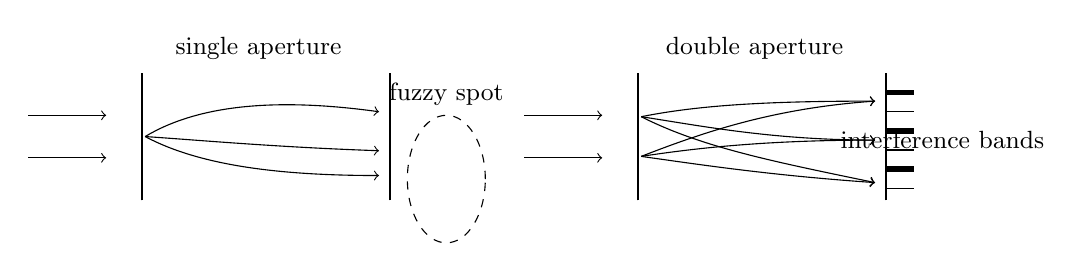
\begin{tikzpicture}[scale=0.9]
\draw[->] (-0.3,1.4) -- (0.8,1.4);
\draw[->] (-0.3,0.8) -- (0.8,0.8);
\draw[thick] (1.3,0.2) -- (1.3,2.0);
\draw[thick,white,line width=5pt] (1.3,1.0) -- (1.3,1.2);
\draw[thick] (1.3,0.2) -- (1.3,2.0);
\draw[thick] (4.8,0.2) -- (4.8,2.0);
\draw[->] (1.35,1.1) .. controls (2.1,1.55) and (3.2,1.65) .. (4.65,1.45);
\draw[->] (1.35,1.1) .. controls (2.1,1.05) and (3.2,0.95) .. (4.65,0.9);
\draw[->] (1.35,1.1) .. controls (2.1,0.7) and (3.2,0.55) .. (4.65,0.55);
\draw[dashed] (5.6,0.5) ellipse (0.55 and 0.9);
\node at (2.95,2.35) {\small single aperture};
\node at (5.6,1.7) {\small fuzzy spot};

\draw[->] (6.7,1.4) -- (7.8,1.4);
\draw[->] (6.7,0.8) -- (7.8,0.8);
\draw[thick] (8.3,0.2) -- (8.3,2.0);
\draw[thick,white,line width=5pt] (8.3,0.75) -- (8.3,0.9);
\draw[thick,white,line width=5pt] (8.3,1.3) -- (8.3,1.45);
\draw[thick] (8.3,0.2) -- (8.3,2.0);
\draw[thick] (11.8,0.2) -- (11.8,2.0);

\draw[->] (8.35,0.82) .. controls (9.2,1.15) and (10.2,1.5) .. (11.65,1.6);
\draw[->] (8.35,0.82) .. controls (9.2,0.95) and (10.2,1.05) .. (11.65,1.05);
\draw[->] (8.35,0.82) .. controls (9.2,0.7) and (10.2,0.55) .. (11.65,0.45);

\draw[->] (8.35,1.38) .. controls (9.2,1.55) and (10.2,1.6) .. (11.65,1.6);
\draw[->] (8.35,1.38) .. controls (9.2,1.25) and (10.2,1.05) .. (11.65,1.05);
\draw[->] (8.35,1.38) .. controls (9.2,0.95) and (10.2,0.75) .. (11.65,0.45);

\draw[line width=2pt] (11.8,1.72) -- (12.2,1.72);
\draw[line width=0.4pt] (11.8,1.45) -- (12.2,1.45);
\draw[line width=2pt] (11.8,1.18) -- (12.2,1.18);
\draw[line width=0.4pt] (11.8,0.91) -- (12.2,0.91);
\draw[line width=2pt] (11.8,0.64) -- (12.2,0.64);
\draw[line width=0.4pt] (11.8,0.37) -- (12.2,0.37);

\node at (9.95,2.35) {\small double aperture};
\node at (12.6,1.05) {\small interference bands};
\end{tikzpicture}
\caption{Single-aperture spreading and double-aperture interference. In the lecture the first effect is suggestive, while the second really nails the wave character of light.}
\end{figure}

This is the point at which the classical wave theory becomes secure. Maxwell then tells us what kind of wave light is: a propagating disturbance of electric and magnetic field. One may picture a wave moving along some axis, with the electric field oscillating transversely and the magnetic field oscillating transversely in a direction perpendicular to the electric field.

\begin{figure}[h]
\centering
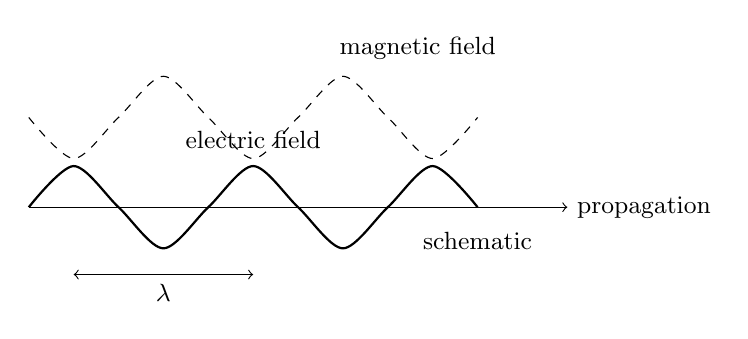
\begin{tikzpicture}[scale=0.95]
\draw[->] (0,0) -- (7.2,0);
\node[right] at (7.2,0) {\small propagation};

\draw[smooth,thick] plot coordinates {(0,0) (0.6,0.55) (1.2,0.0) (1.8,-0.55) (2.4,0.0) (3.0,0.55) (3.6,0.0) (4.2,-0.55) (4.8,0.0) (5.4,0.55) (6.0,0.0)};
\node[above] at (3.0,0.65) {\small electric field};

\draw[smooth,dashed] plot coordinates {(0,1.2) (0.6,0.65) (1.2,1.2) (1.8,1.75) (2.4,1.2) (3.0,0.65) (3.6,1.2) (4.2,1.75) (4.8,1.2) (5.4,0.65) (6.0,1.2)};
\node[above] at (5.2,1.85) {\small magnetic field};

\draw[<->] (0.6,-0.9) -- (3.0,-0.9);
\node[below] at (1.8,-0.9) {\small \(\lambda\)};
\node at (6.0,-0.45) {\small schematic};
\end{tikzpicture}
\caption{A schematic electromagnetic wave. The lecture treats light as a wave of electric and magnetic field before any quantum correction is introduced.}
\end{figure}

Only now, once the classical case is secure, does the lecture slow down and introduce the mathematics of wavelength and frequency.

\section{Wave Kinematics: \texorpdfstring{\(\lambda\), \(T\), \(f\), and \(\omega\)}{lambda, T, f, and omega}}

The first quantity introduced is the wavelength. It is simply the spatial length of one full cycle.

\begin{figure}[h]
\centering

\includegraphics[width=0.72\textwidth]{lecture_01_figure_02.png}
\caption{Introducing \(\lambda\) as the symbol for wavelength. The board writing is only partially visible, but the transcript makes the intended identification clear.}
\end{figure}

We therefore write
\begin{equation}
\lambda = \text{wavelength}.
\end{equation}

The next quantity is temporal rather than spatial. If we stand fixed in place and let the wave pass us, the time for one full cycle is the period, denoted by \(T\). In one period the wave advances one wavelength. Therefore the wave speed is distance divided by time:
\begin{equation}
v = \frac{\lambda}{T}.
\end{equation}
For light, \(v=c\), so
\begin{equation}
c = \frac{\lambda}{T}.
\end{equation}

It is more convenient to replace the period by its inverse, the frequency:
\begin{equation}
f = \frac{1}{T}.
\end{equation}
Substituting into the previous relation gives
\begin{equation}
\lambda f = c.
\end{equation}

\begin{figure}[h]
\centering

\includegraphics[width=0.68\textwidth]{lecture_01_figure_03.png}
\caption{Frequency and wavelength relations on the board. Here the lecture moves from period to frequency and then to the light-wave relation \(\lambda f=c\).}
\end{figure}

The lecture then shifts from cycles per second to the physicists' preferred notation: angular frequency,
\begin{equation}
\omega = 2\pi f.
\end{equation}
The board also shows the equivalent rearrangement \(\omega/(2\pi)=f\). Combining this with \(f=c/\lambda\) yields the central relation
\begin{equation}
\omega = \frac{2\pi c}{\lambda}.
\end{equation}

\begin{figure}[h]
\centering

\includegraphics[width=0.68\textwidth]{lecture_01_figure_04.png}
\caption{The board sequence culminating in the boxed relation \(\omega=\frac{2\pi c}{\lambda}\). The boxed placement marks it as the takeaway equation of the mini-derivation.}
\end{figure}

Let us record the derivation in one line of algebra:
\begin{align}
c &= \frac{\lambda}{T}, &
f &= \frac{1}{T}, &
\lambda f &= c, \nonumber\\
f &= \frac{c}{\lambda}, &
\omega &= 2\pi f, &
\omega &= \frac{2\pi c}{\lambda}. \label{eq:omega-lambda}
\end{align}

This is the point of the notation-heavy pause in the lecture. We are not collecting symbols for their own sake; we are preparing the variables that will shortly enter the photon formulas.

\section{Photons, Blips, and Energy}

\subsection{Question \& Answer}

\paragraph{Question.} If light is a wave, why does it arrive as isolated blips on a screen?

\paragraph{Answer.} The lecture stages this not as a formal theorem but as a practical puzzle. Begin with a beam of light and look at the screen. At ordinary intensity one sees a continuous blob, or, in a two-slit arrangement, a continuous interference pattern. Now attenuate the beam more and more. At some point the character of the observation changes: one no longer sees a smooth illumination, but isolated events, little dots or blips.

If one waits long enough, those discrete arrivals build up exactly the same overall pattern that the classical wave would have produced. The natural conclusion is that light arrives in indivisible units, but the distribution of those arrivals is governed by the wave pattern. In that minimal sense the wave theory becomes a theory of probabilities.

This is the first appearance, in the lecture, of the basic quantum-mechanical compromise: the photon arrives discretely, but the spatial pattern of where it is likely to arrive is wave-like. The same kind of story later appears for electrons. Send electrons through a two-hole arrangement one at a time, and they too build an interference pattern. The lecture pushes the point further: the same phenomenon has been seen even for much larger objects such as buckyballs. So the strange unity of wave and particle is not an eccentric feature of light alone.

Having made that conceptual turn, the lecture immediately asks what a photon carries. The answer is energy, and the energy of a single photon is determined by the frequency:
\begin{equation}
E_\gamma = \hbar \omega.
\end{equation}
Once \(\omega\) has been related to the wavelength, this becomes extremely powerful. From \eqref{eq:omega-lambda} we know that short wavelength means large \(\omega\), and therefore
\begin{equation}
\lambda \downarrow \qquad \Longrightarrow \qquad \omega \uparrow \qquad \Longrightarrow \qquad E_\gamma \uparrow.
\end{equation}

The lecture also insists on a specifically quantum point. A monochromatic beam does not carry an arbitrary continuum of energy. If the beam contains \(n\) photons of the same frequency, then its total energy is
\begin{equation}
E_{\text{beam}} = n\,\hbar\omega,
\qquad
n=0,1,2,\dots
\end{equation}
A radio beam can carry a lot of total energy, but that is because it contains many photons. The energy of each individual long-wavelength photon is small. A gamma-ray photon, by contrast, has a very short wavelength and therefore a much larger energy per photon.

This gives the first clean answer to the question of why smaller structures require bigger machines. If one wants to resolve smaller objects, one needs shorter wavelengths. But shorter wavelengths mean higher frequencies, and higher frequencies mean larger photon energies. The route to the microscopic world therefore runs through energetic probes.

\section{Relativity, Natural Units, and the Return to Momentum}

At this stage the lecture explicitly says that it is not abandoning the previous line of thought. Instead it adds the relativistic side of particle physics. The most famous equation here is
\begin{equation}
E_{\mathrm{rest}} = mc^2,
\end{equation}
but the lecture is careful about modern terminology. We no longer speak of a mass that changes with motion. The modern word \emph{mass} means what older language called \emph{rest mass}. The equation above refers to the energy of a massive object in a frame where the object as a whole is at rest.

Two examples fix the meaning.

First, take a box of gas resting on a scale. If the gas is heated while the box remains at rest, internal energy is added. The lecture's point is that the rest mass of the box increases along with that internal energy. In compact form one may write
\begin{equation}
\Delta E_{\mathrm{rest}} = \Delta m\,c^2.
\end{equation}
The effect is tiny in ordinary units, but the principle is clear: for a body at rest, energy and mass are not different substances; they are the same physical content expressed in different units.

Second, take an electron and a positron at rest and let them annihilate. The rest energy initially stored in the two particles reappears as photon energy:
\begin{equation}
E_{\mathrm{annihilation}} = 2m_e c^2.
\end{equation}
The mechanism may be postponed; energy conservation already forces the conclusion that the rest energy must reappear in some other form.

The lecture then turns to units. Since the numerical value of \(c\) depends on how length and time are measured, one may choose units in which
\begin{equation}
c=1.
\end{equation}
Likewise, since \(\hbar\) is a conversion constant between energy and frequency, one may choose units in which
\begin{equation}
\hbar=1.
\end{equation}
This is not arbitrary cleverness. The lecture's justification is that \(c\) and \(\hbar\) are universal in a very deep sense. The speed of light is a universal limiting speed. Planck's constant is the universal quantum scale that constrains how sharply position and momentum can be specified. Gravity introduces another universal constant, \(G\), but ordinary particle physics is almost entirely insensitive to it, so one usually does not simplify the subject by using Planck units.

\begin{figure}[h]
\centering

\includegraphics[width=0.72\textwidth]{lecture_01_figure_05.png}
\caption{Board evidence for the natural-units form \(E=m\). The visible statement is the simplification of rest energy after setting \(c=1\); the lower handwritten line is too uncertain to promote into a formal equation here.}
\end{figure}

\subsection{Question \& Answer}

\paragraph{Question.} What does \(E=m\) mean, and why is that not the same statement as the photon equation?

\paragraph{Answer.} Once we set \(c=1\), the rest-energy relation simplifies to
\begin{equation}
E_{\mathrm{rest}} = m.
\end{equation}
This does \emph{not} mean that every energy is a mass, or that photons secretly carry rest mass. It means only that for a massive object examined in a frame where it is at rest, the numerical conversion factor between mass and rest energy has been removed by choice of units.

For photons the relevant equation is different. A photon can never be brought to rest, so its energy is not a rest energy. If we also set \(\hbar=1\), then
\begin{equation}
E_\gamma = \omega.
\end{equation}
The two equations are both simplified by natural units, but they refer to different physical situations. The lecture pauses over precisely this point because the notation can otherwise become misleading.

The final closure of the chapter comes when the lecture returns to momentum. For an ordinary slow-moving body, momentum is approximately
\begin{equation}
\mathbf{p} = m\mathbf{v}.
\end{equation}
For light, however, the lecture states a different relation: the magnitude of the momentum of a collimated light beam is its energy divided by \(c\),
\begin{equation}
p = \frac{E}{c}.
\end{equation}
This already explains why the mechanical push of ordinary light is hard to detect: the energy may be measurable, but the extra factor of \(1/c\) makes the momentum small unless the beam is extremely intense.

Now let us do the explicit exercise that ends the mathematical part of the lecture. For one photon,
\begin{align}
p_\gamma &= \frac{E_\gamma}{c} \nonumber\\
&= \frac{\hbar\omega}{c} \nonumber\\
&= \frac{\hbar}{c}\left(\frac{2\pi c}{\lambda}\right) \nonumber\\
&= \frac{2\pi\hbar}{\lambda} \nonumber\\
&= \frac{h}{\lambda}.
\end{align}
Thus the wavelength is not merely a geometrical feature of the wave description. It is directly tied to the momentum of the photon. Shorter wavelength means larger momentum.

We may now combine the lecture's main lines into one chain:
\begin{equation}
\text{smaller structure}
\;\Longrightarrow\;
\text{shorter wavelength}
\;\Longrightarrow\;
\text{larger momentum and energy}
\;\Longrightarrow\;
\text{larger accelerators}.
\end{equation}

This is the practical theme of particle physics as the lecture presents it. If the accelerating gradient is limited, then larger beam energy requires a longer accelerator, at least roughly linearly for a linear machine. One can then ask whether there is any limit to the process of going to shorter and shorter wavelengths. The lecture gives a cautious answer: perhaps the story bottoms out near the Planck length, where gravity and quantum mechanics must be confronted together, but ordinary particle physics remains very far from that scale. Cosmic rays can reach enormous energies, but they arrive with insufficient flux and poor experimental control. So for systematic knowledge we still return to the same principle: build energetic beams, collide them often, and use their short wavelengths to probe smaller structures.

\section{Summary}

The lecture begins with the ancient opposition between particles and continua, and it ends by showing how that opposition is transformed rather than erased. Chemistry gives the first evidence for discreteness. Radioactivity supplies the first particle beam and leads, through the unresolved gamma branch, to light. Light must first be established as a classical wave, and only then may it be recognized as arriving in discrete photons whose probabilities are distributed according to wave patterns.

From there the argument becomes quantitative. Wavelength, period, frequency, and angular frequency are introduced in exactly the order needed to state the photon-energy law \(E_\gamma=\hbar\omega\). Relativity then clarifies the meaning of \(E=mc^2\), natural units strip away arbitrary conversion factors, and the final momentum derivation
\[
p_\gamma = \frac{h}{\lambda}
\]
closes the circle. The shorter the wavelength, the larger the momentum and energy. That is why particle physics advances by building machines that make ever more energetic particles and thereby reveal ever smaller structures.